\documentclass[12pt]{article}
\usepackage{graphicx}
\usepackage[T1]{fontenc}
%\usepackage{lipsum}

\makeatletter
\renewcommand{\maketitle}{\bgroup\setlength{\parindent}{0pt}
\begin{flushleft}
  \textbf{\@title}

  \@author

\end{flushleft}\egroup
}
\makeatother

\title{\large Estimation de performance, Test et Contrôle des Systèmes d’Objets Connectés Utilisant un Réseau de Communication Non-Idéal}
%\title{\large Performance Estimation, Testing, and Control of Cyber-Physical Systems Employing Non-Ideal Communications Networks}
\date{}
\author{%
\ \\
\textbf {Student:} Richard Candell, Universit\'e de Bourgogne, France \& NIST, USA.\\
\textbf{Supervisor:} Sebti Foufou, Universit\'e de Bourgogne, France
}

\pagestyle{empty} % disables page numbers

\begin{document}
\maketitle

% This is samplepaper.tex, a sample chapter demonstrating the
% LLNCS macro package for Springer Computer Science proceedings;
% Version 2.20 of 2017/10/04
%
%---SF- \documentclass[12pt]{article}
%\documentclass[runningheads]{llncs}
%

% Used for displaying a sample figure. If possible, figure files should
% be included in EPS format.
%
% If you use the hyperref package, please uncomment the following line
% to display URLs in blue roman font according to Springer's eBook style:
% \renewcommand\UrlFont{\color{blue}\rmfamily}

%---SF- \begin{document}
	%
%---SF- 	\title{Performance Estimation, Testing, and Control of Cyber-Physical Systems Employing Non-Ideal Communications Networks \\ {\large Extended Abstract}}
	%
	%\titlerunning{Abbreviated paper title}
	% If the paper title is too long for the running head, you can set
	% an abbreviated paper title here
	%
%	\author{Richard Candell\thanks{National Institute of Standards and Technology, United States of America, 100 Bureau Drive, Gaithersburg, MD 20899. \url{http://www.nist.gov}}\\Universit\'e de Bourgogne}
%---SF- \author{
%---SF- {\raggedright
%---SF- 	Student: Richard Candell, Universit\'e de Bourgogne, Dijon, France \& NIST, MD, USA.\\
%---SF- 	
%---SF- 	Supervisor: Sebti Foufou, Universit\'e de Bourgogne, Dijon France
%---SF- }
%---SF- }
	%
%---SF- 	\maketitle            
	%
	\begin{abstract}
		
		La technologie sans fil est un catalyseur clé des promesses de l’industrie 4.0 (fabrication intelligente). En tant que telle, la technologie sans fil sera adoptée comme mode de communication principal au sein de l’usine en général et dans les unités de production en particulier. La communication des unités de production en usine a des exigences particulières en matière de latence, de fiabilité, d’échelle et de sécurité qui doivent d’abord être satisfaites par la technologie de communication sans fil utilisée. Le sans fil est considéré comme une forme de communication non idéale dans la mesure où par rapport aux communications câblées, il est considéré comme moins fiable (avec perte) et moins sécurisé. Ces dégradations possibles entraînent un retard et une perte de données dans un système d’automatisation industrielle où le déterminisme, la sécurité et la sûreté sont considérés comme primordiaux. Cette thèse étudie les exigences d’une communication sans fil dans les unités de production et l’applicabilité de la technologie sans fil existante dans ce domaine. Elle présente une modélisation SysML de l’architecture du système et des flux de données. Elle fournit une méthode d’utilisation des bases de données de type graphe pour l’organisation et l’analyse des données de performance collectées à partir d’un environnement de test. Enfin, la thèse décrit une approche utilisant l’apprentissage automatique pour l’évaluation des performances d’un système d’objets connectés dans le domaine de fabrication. \vspace{2mm}
		
%			Wireless technology is a key enabler of the promises of Industry 4.0 (Smart Manufacturing). As such, wireless technology will be adopted as a principal mode of communication within the factory beginning with the factory enterprise and eventually being adopted for use within the factory workcell.  Factory workcell communication has particular requirements on latency, reliability, scale, and security that must first be met by the wireless communication technology used.  Wireless is considered a non-ideal form of communication in that when compared to its wired counterparts, it is considered less reliable (lossy) and less secure.  These possible impairments lead to delay and loss of data in industrial automation system where determinism, security, and safety is considered paramount.  This thesis investigates the wireless requirements of the factory workcell and applicability of existing wireless technology, it presents a modeling approach to discovery of architecture and data flows using SysML, it provides a method for the use of graph databases to the organization and analysis of performance data collected from a testbed environment, and finally provides an approach to using machine learning in the evaluation of cyberphysical system performance.\vspace{2mm}
		
%			La technologie sans fil est un catalyseur clé des promesses de l'industrie 4.0 (fabrication intelligente). En tant que telle, la technologie sans fil sera adoptée comme mode de communication principal au sein de l'usine, en commençant par l'entreprise d'usine et finalement adoptée pour une utilisation au sein de la cellule de travail de l'usine. La communication des cellules de travail en usine a des exigences particulières en matière de latence, de fiabilité, d'échelle et de sécurité qui doivent d'abord être satisfaites par la technologie de communication sans fil utilisée. Le sans fil est considéré comme une forme de communication non idéale dans la mesure où, par rapport à ses homologues câblés, il est considéré comme moins fiable (avec perte) et moins sécurisé. Ces dégradations possibles entraînent un retard et une perte de données dans un système d'automatisation industrielle où le déterminisme, la sécurité et la sûreté sont considérés comme primordiaux. Cette thèse étudie les exigences sans fil de la cellule de travail de l'usine et l'applicabilité de la technologie sans fil existante, elle présente une approche de modélisation de la découverte de l'architecture et des flux de données à l'aide de SysML, elle fournit une méthode d'utilisation des bases de données graphiques pour l'organisation et l'analyse des données de performance collectés à partir d'un environnement de banc d'essai, et fournit enfin une approche de l'utilisation de l'apprentissage automatique dans l'évaluation des performances du système cyberphysique.
		
%		\keywords{smart manufacturing, industry 4.0, factory communications, wireless, smart manufacturing, test, measurement, machine learning, databases, sysml, abstract modeling.}
		
	\end{abstract}
	%
	%
	%
	
%		Wireless technology is a key enabler of the promises of Industry 4.0 (Smart Manufacturing). As such, wireless technology will be adopted as a principal mode of communication within the factory beginning with the factory enterprise and eventually being adopted for use within the factory workcell.  Factory workcell communication has particular requirements on latency, reliability, scale, and security that must first be met by the wireless communication technology used.  Wireless is considered a non-ideal form of communication in that when compared to its wired counterparts, it is considered less reliable (lossy) and less secure.  These possible impairments lead to delay and loss of data in industrial automation system where determinism, security, and safety is considered paramount.  This thesis investigates the wireless requirements of the factory workcell and applicability of existing wireless technology, it presents a modeling approach to discovery of architecture and data flows using SysML, it provides a method for the use of graph databases to the organization and analysis of performance data collected from a testbed environment, and finally provides an approach to using machine learning in the evaluation of cyberphysical system performance.
	
		\section*{Introduction}
		La fabrication intelligente fournit une vision des futurs systèmes de fabrication qui intègrent des systèmes physiques hautement dynamiques, des systèmes de communication robustes et réactifs et des paradigmes informatiques pour maximiser l'efficacité, permettre la mobilité et réaliser les promesses de l'usine numérique. La technologie sans fil est un catalyseur clé de cette vision. La communication sans fil est intrinsèquement plus sujette à la latence et au retard que ses homologues câblés. De plus, la communication sans fil implique l'utilisation du spectre électromagnétique qui est un support accessible au public avec une capacité limitée et plus sujet aux cyberattaques. Alors que les données transmises peuvent être protégées numériquement par le biais de l'authentification et du cryptage, les appareils sans fil sont sujets aux interférences et au brouillage par des émetteurs voyous et amis, exacerbant les problèmes de fiabilité et de latence affectant les performances de l'usine sans compromettre la sécurité des données. La communication sans fil dans les usines est souvent limitée par la durée de vie de la batterie et très certainement par la disponibilité du spectre électromagnétique. Alors que la dépendance à l'égard des dispositifs sans fil au sein de l'usine se poursuit, des étapes vers le développement d'un réseau de communications sans fil plus robuste doivent être développées. Ces étapes comprennent:
			
		\begin{itemize}
			\item[$\star$] Le système d'automatisation doit devenir sensible à la situation et s'adapter à la connaissance des tendances de l'occupation du spectre électromagnétique et des événements aigus; et
			
			\item[$\star$] L'intelligence du système d'automatisation doit se rapprocher du système physique. Cela signifie déplacer l'intelligence pour le contrôle vers l'actionneur; et
			
			\item[$\star$] Des méthodes d'essai de performance doivent être développées et incorporées dans les dispositifs à franges industriels. Les méthodes d'essai doivent être fiables et en même temps faciles à utiliser par un personnel d'usine non formé aux techniques de la communication sans fil; et
			
			\item[$\star$] Les protocoles de communication sans fil existants doivent être analysés et adaptés, et de nouveaux protocoles doivent être développés pour équilibrer la fiabilité, la latence et l'évolutivité; et
			 
			\item[$\star$] La sécurité du réseau doit être maintenue et doit inclure la disponibilité comme caractéristique primordiale.
		\end{itemize}
		
		Cette thèse comprend le développement d'approches de test pour mesurer les performances des réseaux sans fil industriels déployés dans des cellules de travail de fabrication intelligentes. Ainsi, l'objectif principal de cette thèse est la découverte de méthodes et d'approches pour l'évaluation des performances des cas d'utilisation industrielle pour les cas d'utilisation dans lesquels la technologie de communication sans fil est utilisée comme mode de communication principal. La principale motivation de la recherche est de découvrir des méthodes d'essai et d'évaluation pratiques pour évaluer les performances d'une cellule de travail industrielle, améliorant ainsi la sécurité, la sûreté et la fiabilité en général. Les résultats et les résultats du travail de thèse sont inclus dans la thèse et publiés en tant qu'articles de journaux et actes de conférence. Les données résultantes sont également mises à disposition.
		
		\section*{Contributions et organisation}
		
		Cette thèse est présentée en trois grandes parties. Dans la partie I, la thèse fournit une introduction historique au contexte de la fabrication intelligente. Il présente les prémisses de la technologie sans fil industrielle, les principaux défis de l'utilisation du sans fil dans un environnement d'usine et les indicateurs acceptés qui sont actuellement utilisés dans l'application du sans fil dans les environnements d'usine. Ensuite, l'état actuel de la technique est présenté pour orienter le lecteur vers la contribution de la thèse. Cet état de l'art comprend une discussion sur le paysage de la technologie sans fil industrielle, les normes et une cartographie provisoire de ces technologies dans les domaines d'application. Une discussion des approches de modélisation des systèmes est ensuite fournie avec un accent sur le langage de balisage des systèmes. Ensuite, une discussion sur les approches de l'utilisation des bases de données suit. Dans la partie II, \ textit {Thesis Contributions}, les contributions techniques de cette thèse sont présentées. Enfin, dans la partie III, la thèse fournit une discussion détaillée des quatre principales contributions de ce travail de thèse. Les remarques finales et l'orientation future sont fournies en tant qu'avis du candidat à la thèse. Les contributions de thèse sont présentées comme suit:\vspace{5mm}
		
		\begin{description}
			
			\item[Exigences]
			\cite{CandellRW2017} \cite{Montgomery2019} \cite{Candell2018.IWSGuide} \cite{ieeeMagazine2018} Un examen du paysage de la technologie sans fil est effectué. Les technologies sans fil existantes et futures sont évaluées pour leur applicabilité appropriée aux cas d'utilisation industrielle.
			
			\item[La modélisation] \cite{Candell2019ASR.SYSML} \cite{Candell2018SysML.JRES} Afin de mieux comprendre la composition architecturale de la cellule de travail à l'aide de la communication sans fil industrielle, des techniques de modélisation sont utilisées pour identifier et décomposer les pièces, les interfaces et les flux de données. SysML est adopté pour ce processus et une bibliothèque de modélisation proposée est créée et présentée. Le modèle avec diagramme conceptuel est rendu public indépendamment de l'outil qui a été utilisé pour créer le modèle.
			
			\item[Application de la base de données Graph] \cite{CandellISIT2020.Conf} Une méthode est développée pour collecter, nettoyer, organiser et présenter les indicateurs de performance cyberphysiques des expériences menées dans le banc d'essai sans fil industriel NIST. La méthode développée utilise la base de données de graphes Neo4j et est présentée comme une nouvelle approche par rapport aux approches traditionnelles utilisant une base de données relationnelle, des feuilles de calcul et un traitement de fichiers bruts.
			
			\item[Apprentissage automatique] \cite{CandellISIE2019.Conf} \cite{CandellIJAMT2020.Jrnl} Une technique d'apprentissage automatique est développée et appliquée à la prédiction des niveaux de signal à interférence dans un réseau de cellules de travail sans fil utilisant un bras de robot dans un appareil de recherche de force. La méthode d'apprentissage automatique permet à un réseau entraîné de déterminer avec précision le niveau signal-interférence en utilisant l'état physique du bras du robot plutôt que l'état de la liaison sans fil elle-même.
			
		\end{description}
	
		L'auteur cite également son article~\cite{Candell.PLMConf2020} soumis à une prochaine conférence sur la gestion du cycle de vie des produits. L'auteur présente une nouvelle conception de banc d'essai sans fil industriel qui motive la recherche universitaire et répond aux besoins de l'industrie. Le banc d'essai est conçu pour servir à la fois de plate-forme de démonstration et de recherche pour la cellule de travail sans fil. Le travail s'appuie sur les enseignements tirés des incarnations passées, notamment un scénario de maintenance de machine à double robot et un appareil de bras de robot à recherche de force et de couple. Cette version du banc d'essai comprend des éléments de calcul et de communication tels que le fonctionnement du système physique est sensiblement dégradé sous l'influence des interférences radio, du trafic réseau concurrent et des effets de propagation radio appliqués dans le laboratoire. Les principaux indicateurs de performance du banc d'essai sont sélectionnés et présentés, notamment les indicateurs des systèmes de communication, de calcul et physiques. Ce nouveau banc d'essai sera utilisé pour effectuer de futures recherches motivées par cette thèse.
		
		Une contribution supplémentaire de l'auteur pour laquelle il n'était pas l'auteur principal mais a joué un rôle important est citée ici~\cite{MSEC2019-2896}.  Dans ce travail, l'auteur a conçu, construit et exécuté une expérience en collaboration avec l'auteur principal dans laquelle un appareil de portique bidimensionnel typique était contrôlé par un contrôleur local qui recevait des commandes de code G sans fil sur un réseau Wi-Fi. Le canal sans fil industriel a été reproduit à l'aide d'un émulateur de canal radiofréquence (RF) où divers scénarios ont été envisagés et divers paramètres de canal sans fil ont été étudiés. Le mouvement de l'outil du système de portique a été suivi à l'aide d'un système de suivi de la vision pour quantifier l'impact du canal sans fil sur les performances du système. Des résultats numériques ont été présentés, y compris le temps d'exécution total d'un processus industriel et les temps de séjour à différentes positions tout au long du processus. Cette contribution n'est pas discutée dans la thèse.


%		\section{Industrial Wireless Technology and Applications}
%		
%		\section{Workcell Architectural Decomposition}
%		
%		\section{Application of Graph Databases}
%		
%		\section{Application of Machine Learning}
		
\section*{Cartographie des exigences}

La première contribution a été une exposition des différentes technologies sans fil qui ont été développées spécifiquement pour un usage industriel ou qui ont une utilisation tangentielle dans l'industrie. Des classes de cas d'utilisation industrielle ont été définies et une cartographie de l'applicabilité de chaque technologie sans fil à la classe de cas d'utilisation a été fournie. Cette cartographie représentait l'opinion du candidat sur la base de son expérience et de ses connaissances de la technologie sans fil au moment de la contribution. Cette exploration a représenté une contribution majeure à la distillation de la pléthore d'exigences de performance trouvées dans la littérature et dans les articles commerciaux concernant les attentes de performance des réseaux sans fil industriels et les exigences de conduite derrière les cas d'utilisation qui les utilisent. Dans cet article, des considérations de réussite sont présentées pour le déploiement du sans fil dans les usines et les cellules de travail en usine, y compris celles envisagées pour la fabrication intelligente. Ces considérations de réussite sont définies et incluent la fiabilité. L'indicateur de performance \ textit {fiabilité} est une considération principale dans cette thèse et représente l'essentiel des préoccupations pour les déploiements sans fil. La fiabilité comprend tout élément ayant un impact sur le flux d'informations au sein d'un système cyberphysique. Cela inclut à la fois la perte et le retard des informations. Dans cette contribution, plusieurs composants comprennent l'espace problématique des déploiements sans fil dont deux résonnent d'une importance critique pour les travaux traités par cette thèse. Le premier est le problème de l'instrumentation qui comprend tous les éléments de l'usine qui incluent la détection et l'actionnement. Le deuxième élément important est l'évaluation des performances qui comprend des méthodes de test pour lesquelles cette thèse aborde à travers l'identification des flux d'informations, puis l'évaluation des performances de ces flux d'informations et de leurs impacts sur les performances physiques. Par conséquent, cette contribution est nécessairement importante car elle fournit une perspective essentielle du problème du déploiement de systèmes sans fil industriels, puis de la motivation derrière la modélisation, l'application de base de données et l'apprentissage automatique pour l'évaluation des performances du réseau. La contribution de ce travail illustre le besoin clair de comprendre les exigences et les méthodes de test créatives pour l'examen des systèmes cyberphysiques sans fil. Il ressortait clairement de cette contribution que des méthodes d'essai faciles à utiliser étaient essentielles; cependant, ce n'était pas un objectif de cette thèse. Essentiellement, cette contribution pose le problème de la sélection et du déploiement de réseaux sans fil dans les usines. Il décrit les aspects techniques à considérer. Enfin, il fournit un point de départ pour l'applicabilité des technologies sans fil à des classes de cas d'utilisation et, ce faisant, fournit une motivation pour acquérir une meilleure compréhension de la cellule de travail grâce à une décomposition formelle et à la création d'un cadre pour communiquer ces idées.

\section*{Modélisation à l'aide de SysML}
La deuxième contribution était une abstraction du système cyberphysique industriel qui est le travail en usine utilisant SysML. Dans ce travail, un modèle a été construit en utilisant des primitives représentant chaque composant architectural majeur de la cellule de travail et les interfaces à l'intérieur de la cellule de travail et aux systèmes à l'extérieur de la cellule de travail. Ces interfaces sont utilisées pour représenter des éléments du flux d'informations. Les flux d'informations représentés représentent les performances du réseau support. Par la suite, le système physique qui fonctionne en utilisant ce réseau a ses propres performances qui sont directement connectées aux performances du réseau. Chaque flux d'information identifié à l'aide du modèle SysML représente une opportunité d'étude. Par exemple, le système élaboré par le schéma fonctionnel interne Fig.~\ref{fig:concl:lfscenario-full} chacun des principaux acteurs (Robot Controller 1, Robot Controller 2 et Supervisor) sont tous connectés à un réseau 802.11ax.

\begin{figure}[!th]
	\centering
	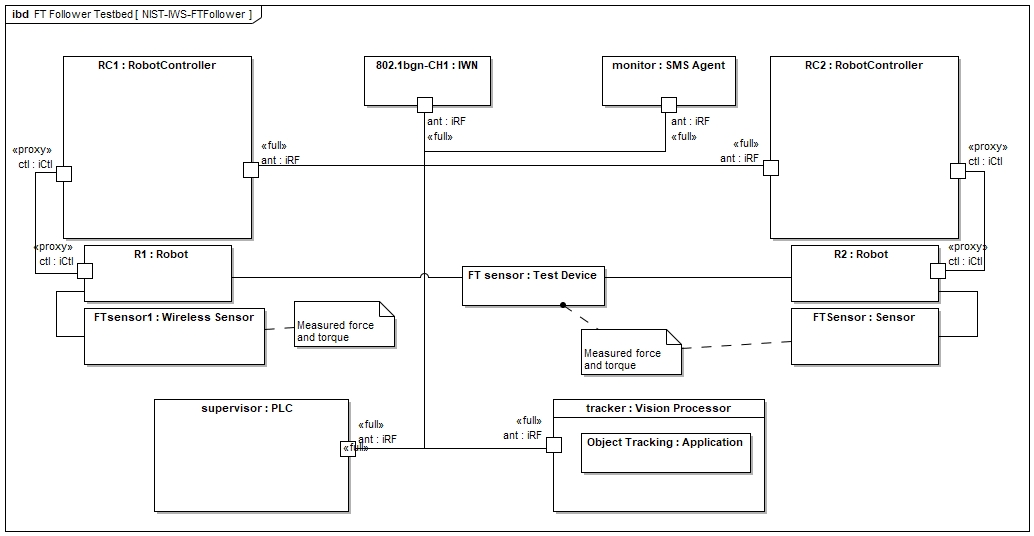
\includegraphics[width=0.95\textwidth]{../chapter-conclusions/images/NIST-IWS-FTFollower}
	\caption{Schéma fonctionnel interne d'une cellule de travail équipée d'une application de levage robot-suiveur.}
	\label{fig:concl:lfscenario-full}
\end{figure}
%
%\begin{figure}[!th]
%	\centering
%	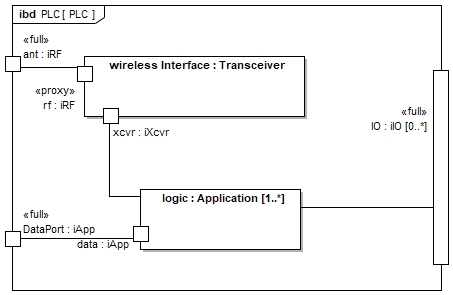
\includegraphics[width=0.85\textwidth]{../chapter-conclusions/images/PLC}
%	\caption{Internal block diagram of a PLC.}
%	\label{fig:concl:plc-ibd}
%\end{figure}
%
%\begin{figure}[!th]
%	\centering
%	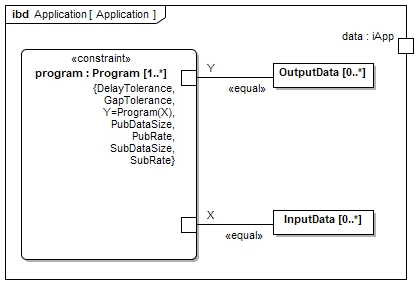
\includegraphics[width=0.85\textwidth]{../chapter-conclusions/images/Application}
%	\caption{Internal block diagram of an Application showing the parametrics constraints of its one or more programs.}
%	\label{fig:concl:Application-ibd}
%\end{figure}
%
%\begin{figure}[!th]
%	\centering
%	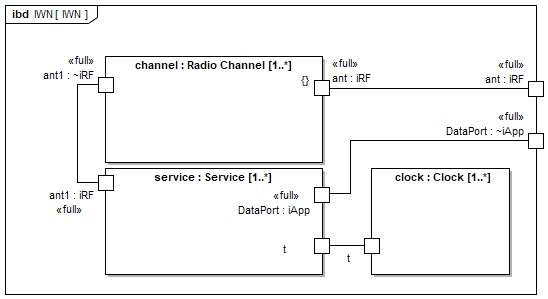
\includegraphics[width=0.85\textwidth]{../chapter-conclusions/images/IWN}
%	\caption{Internal block diagram of an Industrial Wireless Network (IWN) showing the parametric constraints of its one or more programs.}
%	\label{fig:concl:iwn-ibd}
%\end{figure}
%
%\begin{figure}[!th]
%	\centering
%	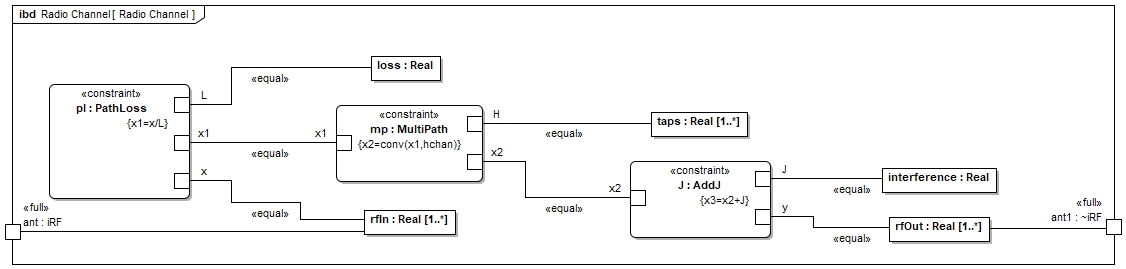
\includegraphics[width=0.85\textwidth]{../chapter-conclusions/images/RadioChannel}
%	\caption{Internal block diagram of an Radio Channel showing the parametric constraints of the radio medium.}
%	\label{fig:concl:RadioChannel-ibd}
%\end{figure}
%
%\begin{figure}[!th]
%	\centering
%	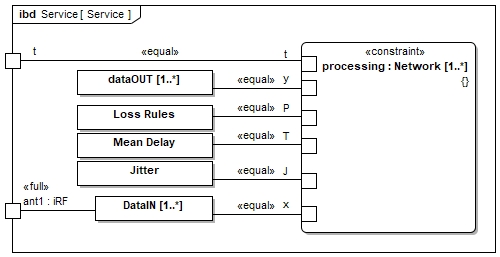
\includegraphics[width=0.85\textwidth]{../chapter-conclusions/images/Service}
%	\caption{Internal block diagram of an IWN Service showing the parametric constraints of the behavior of a network service as generic processing.}
%	\label{fig:concl:Service-ibd}
%\end{figure}

%And as shown in Fig.~\ref{fig:concl:conceptual}, each controller block such as a Robot Controller or a PLC~(Fig.~\ref{fig:concl:plc-ibd}) inherits its structure and behavior from the Controller block.  As such, the PLC and the Robot Controller have an Application and an interface the to the wireless network.  Each application is linked to the wireless network through a Transceiver block (refer to \ref{fig:concl:plc-ibd}) which intuitively governs its own receiver performance as impacted by the radio channel.  The radio channel is an element of the IWN block shown in Fig.~\ref{fig:concl:iwn-ibd} which is connected directly to a set of IWN services as shown in Fig.~\ref{fig:concl:Service-ibd}. The service block of the IWN is modeled as a generic sets of contraints that could be implemented as code or mathemetical limitations.  

On peut clairement voir que le chemin complet du flux d'informations dans le modèle proposé traverse le support radio, le réseau sans fil industriel, les émetteurs-récepteurs embarqués et chaque application de contrôle. Par conséquent, il est possible d'utiliser ce modèle proposé pour représenter le canal radio, modéliser ses impacts sur les performances du réseau sans fil, et par la suite les impacts des performances du réseau sans fil sur les performances des applications de contrôle elles-mêmes. Ce n'est pas une perspective facile et pourrait être très difficile pour un ingénieur qui tente de le faire; cependant avec le modèle présenté, c'est tout à fait possible. Cela représente une opportunité pour affiner le modèle proposé pour être plus intuitif et peut-être plus facile à utiliser.  

\begin{figure}[!th]
	\centering
	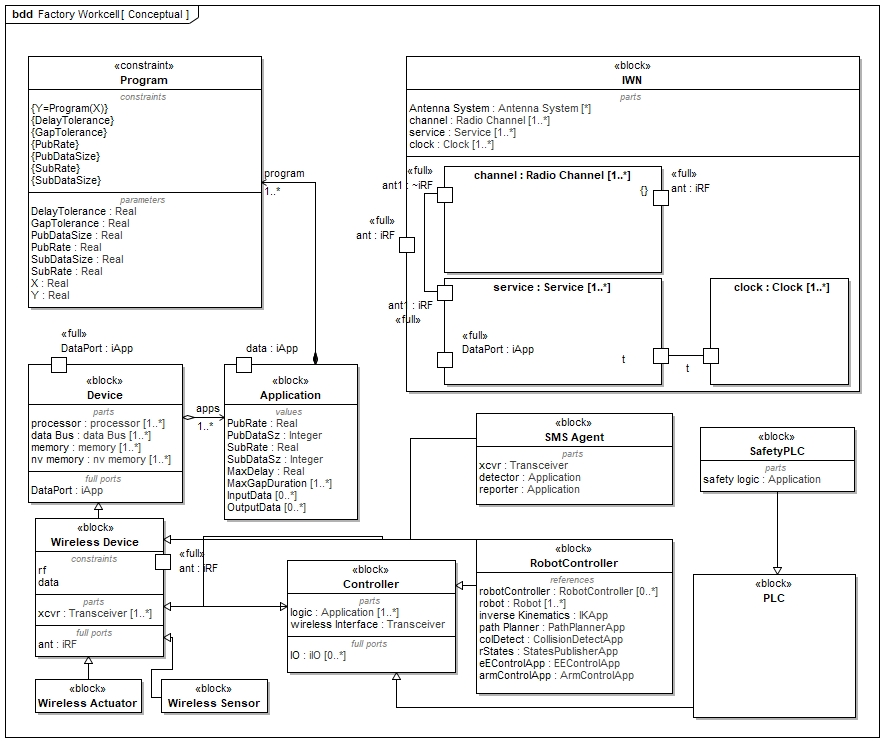
\includegraphics[width=0.95\textwidth]{../chapter-conclusions/images/Conceptual}
	\caption{BBD des relations conceptuelles des primitives de modèle.}
	\label{fig:concl:conceptual}
\end{figure}

%A model was developed using SysML. The developed model is constructed of the elements necessary to construct useful representations of factory work-cells in which wireless networks are used to transport information necessary for automated control system operation.  Reusable, derivable elements are developed and then extended to represent the constructs of the work-cell such as robot control, supervisory control, vision, safety, and spectrum monitoring.  An industrial wireless network is then developed and constraints of the radio channel and network services are formalized. Using the architectural model, information flows are explored and incorporated within. 
%
%It is important to mention that this model includes an often overlooked component of any industrial wireless deployment which is the spectrum monitoring system and also considers the human-robot and robot-robot interactions in industrial environments. The current model includes various systems constraints including motion constraints, radio channel constraints, and networking constraints. The parametric constraints are provided as examples and can be replaced with executable computer code thereby making the model useful for simulation depending on the modeling tool selected. Furthermore, the applications within the robotic work-cell define many information flows requiring careful analysis to achieve reliability and latency necessary for the safety and control of the manufacturing process.

Avec une dépendance accrue aux communications sans fil pour des systèmes de fabrication plus complexes, la projection des exigences de fabrication sur le système de communication sans fil devient moins évidente. Une telle analyse de cette projection est essentielle pour la recherche future des systèmes de fabrication. A ce titre, les éléments architecturaux et les flux d'informations exposés par un modèle abstrait
sont une première étape nécessaire. Le modèle dans son état actuel de développement est suffisamment complet pour prendre en charge les analyses architecturales et ontologiques de la cellule de travail de l'usine. En tant que tel, des informations sur les relations entre les composants d'une cellule de travail et les attributs liés au réseau sans fil peuvent être découvertes. Par conséquent, le modèle sert de base aux futures analyses d'ingénierie des systèmes. De plus, le modèle peut être utilisé comme un outil d'exploration académique et industrielle du développement de bancs d'essai sans fil.  

\section*{Application de base de données graphique}

Les bases de données graphiques sont conçues pour fournir un cadre de modélisation puissant pour le stockage et la visualisation des données dans lesquelles les relations et les connexions entre les données peuvent être importantes mais difficiles à détecter ou à visualiser dans le monde réel. Quand on entend le mot «base de données», on imagine généralement une base de données relationnelle telle que MySQL ou Oralce dans laquelle la base de données elle-même stocke les informations d'une manière hautement structurée dans laquelle les tables sont construites d'une manière prédéterminée avec des colonnes, des lignes et des données définies de manière rigide les types. En revanche, les bases de données graphiques ne sont pas rigides dans leur structure et leur organisation. Les données sont des bases de données graphiques qui sont nativement stockées dans des nœuds et des sommets (connexions). Chaque nœud et sommet peut avoir des propriétés associées et ainsi stocker des données. Dans le graphique, il existe des unités d'informations (nœuds) avec des lignes de relations entre ces unités d'informations représentées sous forme de lignes. Les lignes de connexion entre les nœuds représentent des relations qui sont le bloc de construction essentiel utilisé dans la contribution présentée dans la thèse.
%as shown in Fig.~\ref{fig:concl:graphdb-sperical} which illustrates the common notion of a graph database.  
%In the graph, units of information (nodes) exist with relationships lines between those units of information depicted as lines.  The connecting lines between nodes represent relationships which are the essential building block used within the contribution presented in the thesis~\cite{CandellISIT2020.Conf}.  

%\begin{figure}[!ht]
%	\centering
%	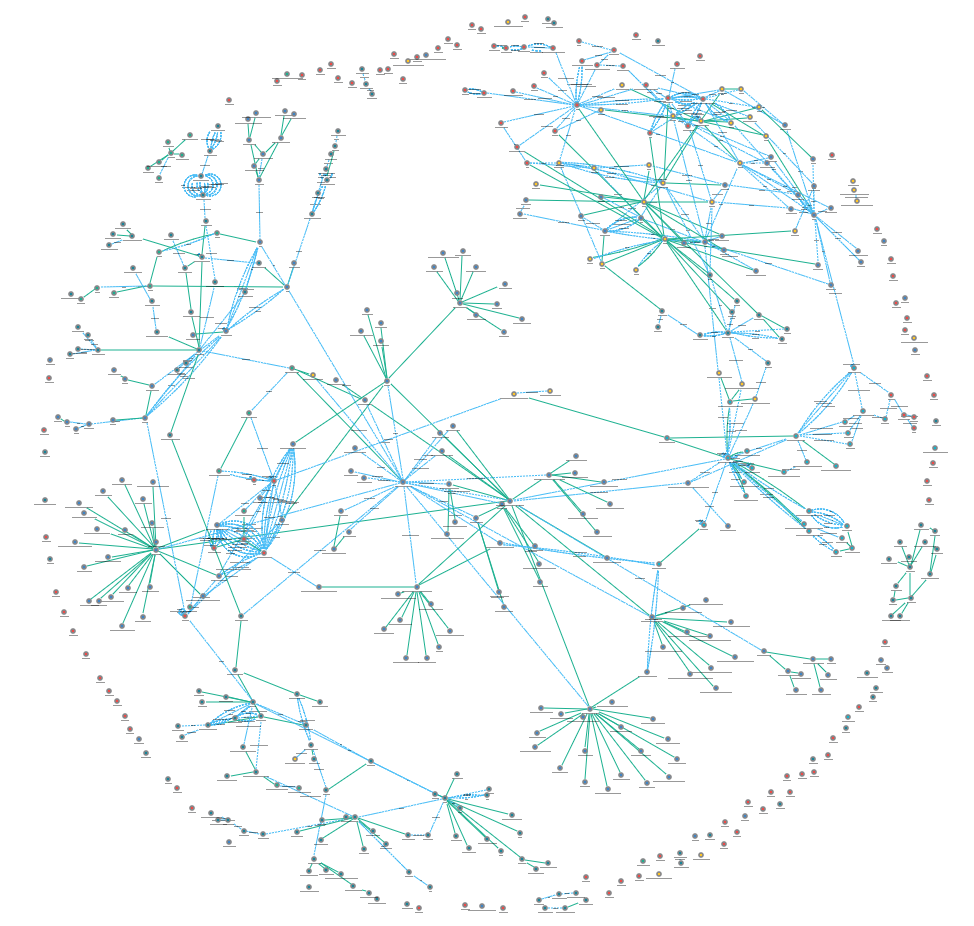
\includegraphics[width=0.4\textwidth]{../chapter-conclusions/images/spherical-graph.png}
%	\caption{A notional spherical graph depicting nodes and vertices.}
%	\label{fig:concl:graphdb-sperical}
%\end{figure}

La base de données graphique a été utilisée dans le cadre de cette thèse. Il a été démontré comme un outil efficace pour modéliser et capturer des informations sur les performances pour la recherche et éventuellement pour la connaissance de la situation du fonctionnement de l'usine. L'objectif de l'utilisation d'une base de données graphique était essentiellement de 1) tirer parti de la connectivité inhérente aux données résultant des expériences menées au sein du NIST Industrial Wireless Laboratory, et 2) démontrer que les réseaux sans fil pouvaient être utilisés pour une classe significative de cas d'utilisation sans impact sur les performances du système physique. Pour soutenir les recherches effectuées pour cette contribution, un banc d'essai a été construit. Deux bras de robot ont été utilisés pour déplacer et inspecter les pièces à travers une série de quatre (4) machines à commande numérique par ordinateur (CNC). Chaque robot est équipé d'un capteur de couple de force 6 DOF dans son poignet. Le contrôle conjoint de chaque robot est effectué via un ensemble informatique de contrôleur de robot séparé. Un contrôleur logique programmable (PLC) a été utilisé pour superviser l'activité au sein de la cellule de travail et a été appelé le superviseur. Le réseau et les performances physiques de la cellule de travail simulée ont été capturés complètement indépendamment du type de réseau de communication utilisé. Grâce à l'adaptateur et aux dispositifs de prise réseau illustrés dans le diagramme, il a été possible de capturer les données de vol par paquets de telle sorte que le type de technologie utilisé pour la communication ne modifie pas le routage des informations. Ce faisant, le schéma du graphique basé sur les données est resté relativement inchangé entre les expériences tandis que différents protocoles filaires et sans fil ont été étudiés. De nombreuses instanciations de bases de données graphiques ont été produites pour chaque expérience réalisée à l'aide du banc d'essai.  

%\begin{figure}[!ht]
%	\centering
%	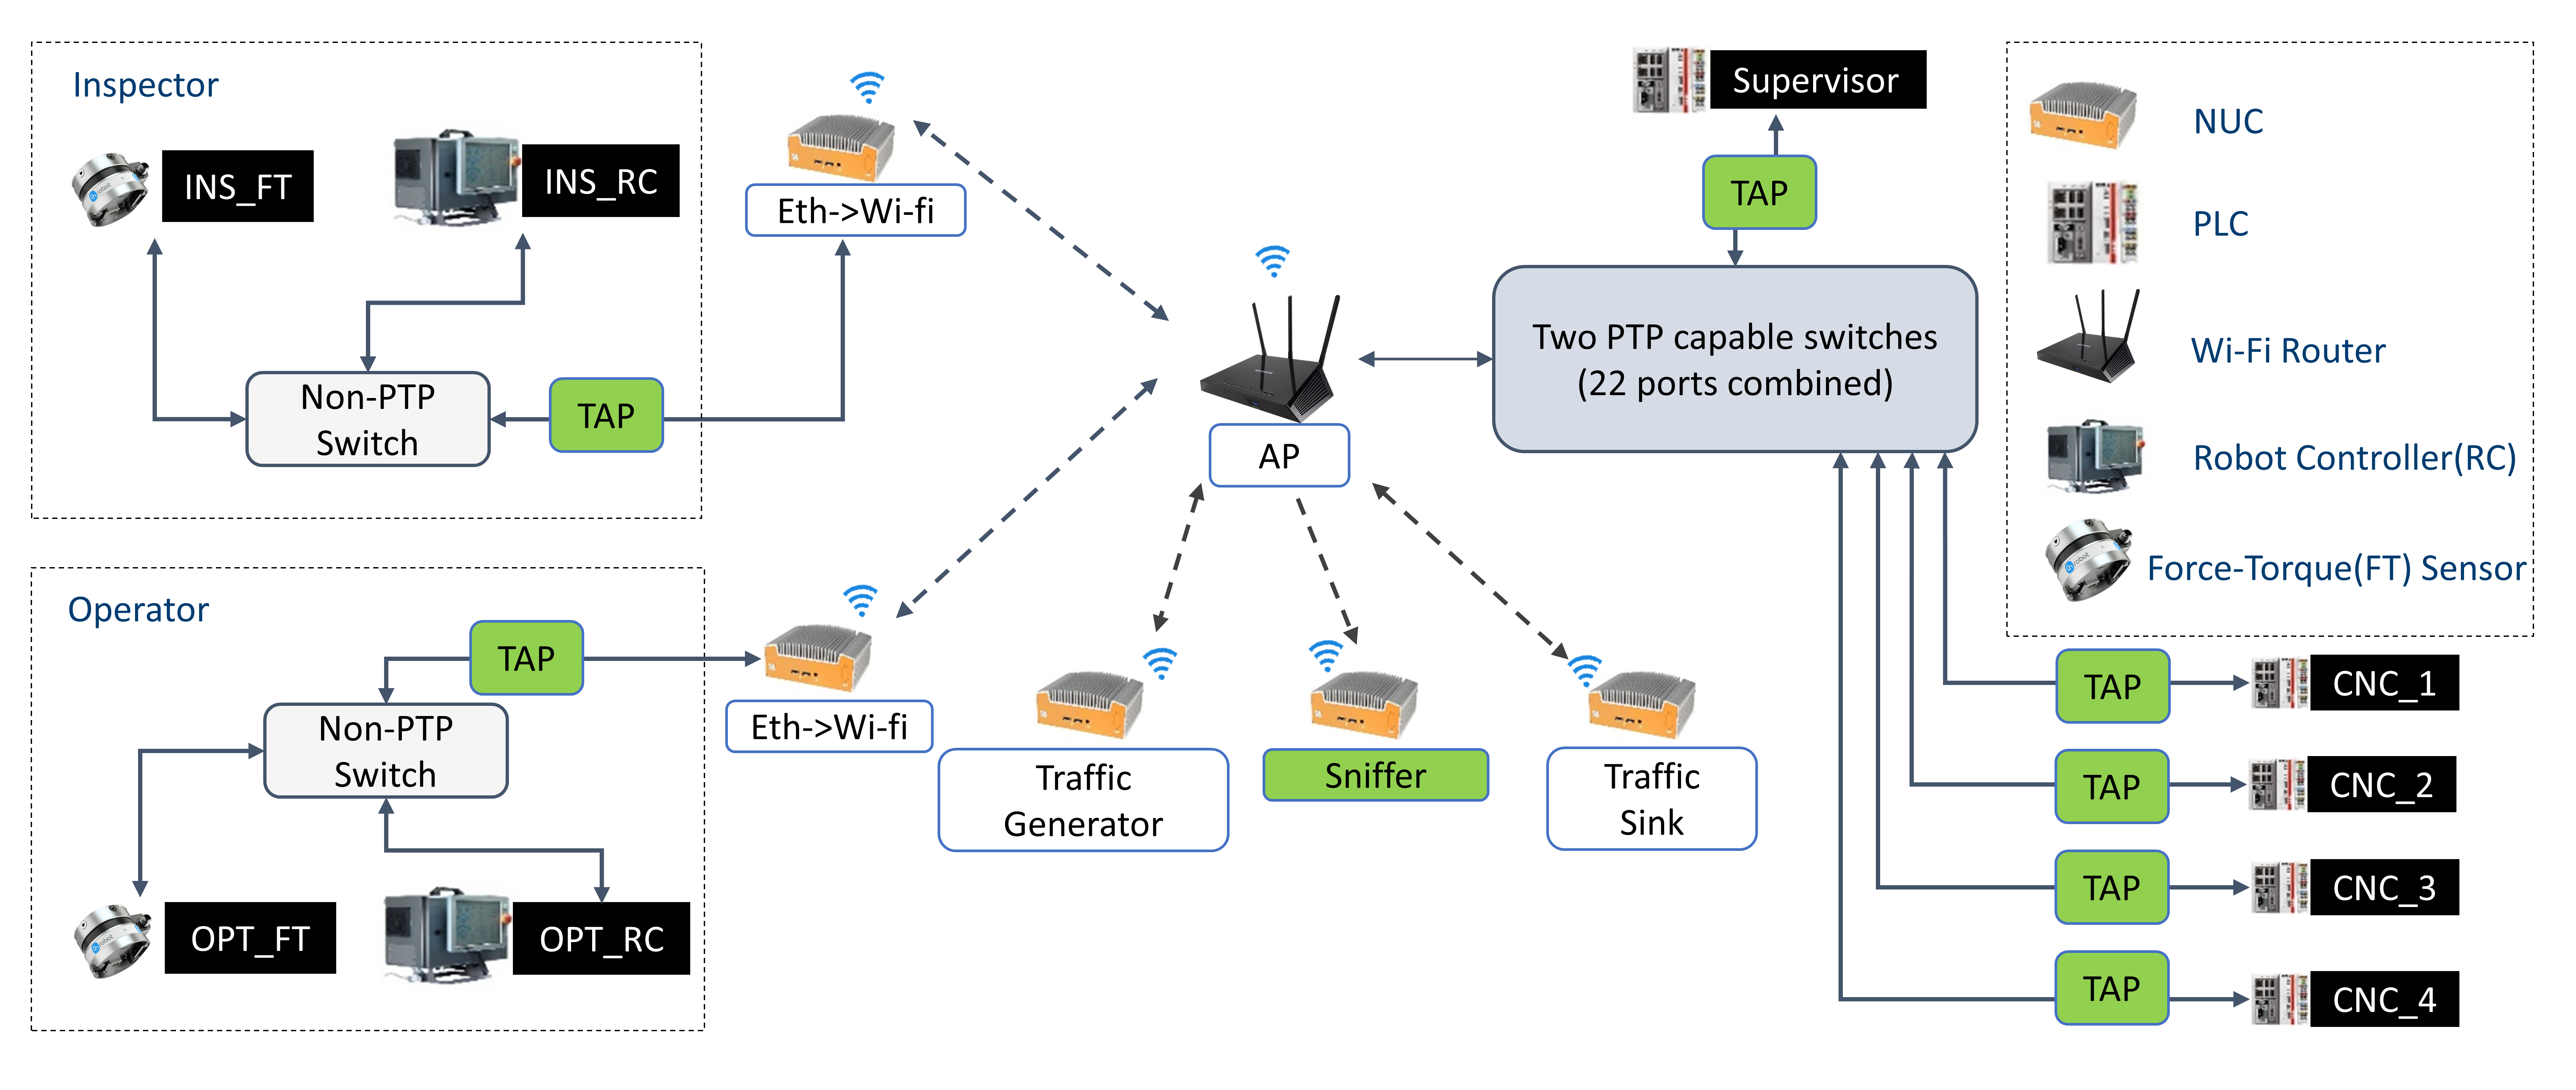
\includegraphics[width=0.95\textwidth]{../chapter-gdb-appl/figures/Fig1TiiSpecialDiagram-testbed2.png}
%	\caption{Experiment design used for capture of performance data.}
%	\label{fig:concl:experiment-design}
%\end{figure}
%
%This shows what is important: the connection between physical actions that the transactions that support them.  Transactions are grouping of information transmissions (i.e., packets) that traverse the wireless network.  Factors that impact reliability of transaction such as message (i.e. packet) loss or message (i.e. packet) delay indirectly impact start and stop times of physical actions.  These relationships are directly captured within a graph and thus the applicability of a graph database to the investigation of cyberphysical system performance becomes evident.  Ultimately, one could argue that the primary contribution of this component of the thesis is the demonstration of interconnectedness between the industrial (wireless) network and physical operations through the modeling and capture of the performance data, the data relationships, and the analysis of physical action performance when network performance is degraded.  The use of the graph database makes that possible.  As an example, the schema shown in Fig.~\ref{fig:concl:data-physical-actions-following} was produced by querying the schema of a single database with hundreds of physical actions and hundreds of thousands of supporting transactions.  By querying the data represented by this structure, it was demonstrated that the wireless network employed did not prohibitively impact operation.  It was also demonstrated that through querying of the performance outliers that network events such as loss in signal strength or an increase in interference could be linked to a delay in the actuation of a robot action.  This type of event discover and correlation to the physical world is particularly advantageous to facilitating the adoption of wireless in smart manufacturing.

%\begin{figure}[!ht]
%	\centering
%	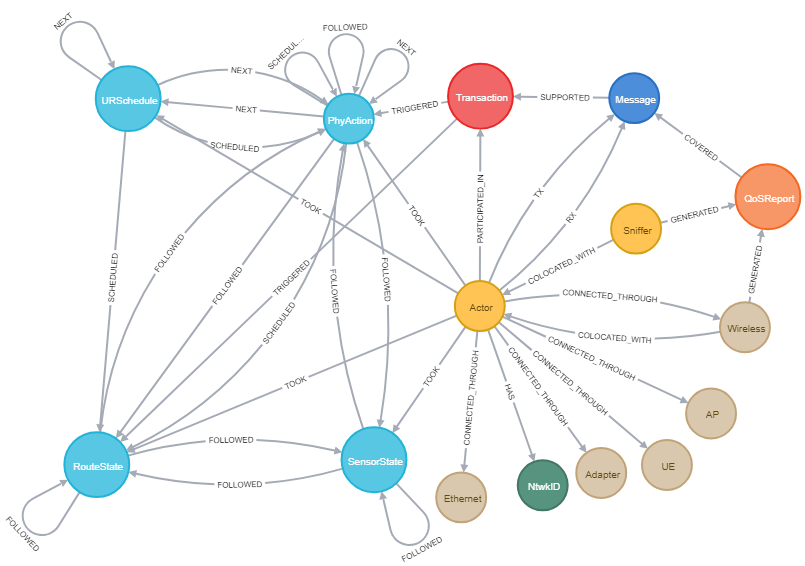
\includegraphics[width=0.85\textwidth]{../chapter-gdb-appl/figures/database/graph_schema_updated_2.png}
%	\caption{Experiment design used for capture of performance data.}
%	\label{fig:concl:data-physical-actions-following}
%\end{figure}
%
%It is my opinion that the relationships between the physical actions through the FOLLOWED and NEXT relationships as shown in Fig.~\ref{fig:concl:data-physical-actions-following} and the TRIGGER relationships between physical actions and Transcactions present a signifcant component of discovery within the results of this contribution. It is through the TRIGGER and FOLLOWED relationships that one can ascertain the impacts of network performance on physical systems performance. These are difficult to model with relationship databases.  It is possible to so so, but it is not inherent in the nature of the database itself to store such relationships.  When a triggering Transaction is correlated to a physical action using these relationships, it is then possible to follow the nodes backward in the graph to associated Message nodes and the quality of service (QoS) reports associated with those messages. These QoS reports provide evidence of degradation within the communication network during operation.  It is important to note that the QoS reports used for this investigation were produced externally using wireless sniffer devices that were co-located with transceiver equipment.  This was done due to the implementation difficulty in extracting QoS header information for each wireless packet received at each actor.  Since the experiments were performed, a method to extract wireless QoS header data at each transceiver was discovered.  Capture of wireless header information would enrich the data with more accurate QoS reports applicable directly to informational messages and thus allow for the construction of a more accurate data graph.

\section*{Applications d'apprentissage automatique}

L'apprentissage automatique est ce vaste domaine de la science et de l'ingénierie qui traite de l'application d'algorithmes de calcul pour effectuer des actions sans être explicitement programmé pour le faire. Dans les applications générales, l'apprentissage automatique est utilisé à partir d'applications allant de la reconnaissance vocale dans l'électronique personnelle, le filtrage du spam dans les e-mails, et la réalisation de prévisions de trafic pour les navetteurs à la fourniture de services tels que l'identification des amis et la reconnaissance faciale dans les médias sociaux. Dans les applications industrielles, l'apprentissage automatique a la promesse d'un large éventail d'applications telles que l'autonomie des robots et la détection des anomalies de sécurité. Dans cette thèse, un cadre d'apprentissage automatique a été démontré pour la prédiction du rapport signal / interférence dans une liaison de communication utilisée pour la commande d'un bras de robot enfonçant un appareil à ressort. Le cadre ML s'est révélé utile et précis dans la prédiction de la qualité de la liaison. L'estimation de la qualité de la liaison est une mesure importante dans le système de communication sans fil. Il s'agit d'un terme général utilisé pour décrire le niveau de qualité d'un lien de communication. La métrique du rapport signal / brouillage est un rapport entre le signal prévu transmis et le niveau d'interférence en concurrence avec le signal prévu. Les interférences, qu'elles soient causées par un brouillage malveillant ou non, sont un facteur entravant l'adoption du sans fil dans les systèmes de fabrication intelligents. Par conséquent, il est clairement intéressant d'avoir une image claire de la conscience de la situation du niveau d'interférence et de la qualité des liaisons de communication utilisées. La contribution présentée dans cette thèse répond à un besoin évident d'améliorer la détection et l'estimation des événements de qualité du signal dans la cellule de travail.  

%Future work to extend the framework could involve the following:
%
%\begin{description}
%	
%	\item[Higher Dimensionality] Application of this ML framework to a system with more degrees of freedom such as the entire workcell.  In the current contribution, the ML framework was applied to a single wireless communication link used to control one robot arm.  When expanded the framework to systems with more dimensions, the application of neural networks with deep learning may be beneficial.
%	
%	\item[Spectrum Monitoring System] Application of online learning techniques such that the ML framework can learn and adapt as the workcell operates would be beneficial as well.  In the current contribution, the ML framework learns offline from training data and then applies its knowledge to an active system.  This prohibits the system from learning as the wireless network changes over time.  Online techniques could allow for the ML framework to account for a changing spectral environment.
%	
%	\item[Control System Integration] Integration of this framework with the workcell control system such that the control system can adapt dynamically to interference for example to allow the control system to task preventative actions for safety or to operate in a reduced performance mode.
%	
%\end{description}

	
		


		\bibliographystyle{IEEEtran}		
		\bibliography{bibliography} 

	
	


%\begin{biography}[{\includegraphics[width=1in,height=1.25in,clip,keepaspectratio]{mshell}}]{Michael Shell}
% or if you just want to reserve a space for a photo:

%\begin{IEEEbiography}[{\includegraphics[width=1in,height=1.25in,clip,keepaspectratio]{liuyk}}]{Yongkang Liu}
%is currently working toward a Ph.D. degree with the Department of Electrical
%and Computer Engineering, University of Waterloo, Canada. He is currently a
%research assistant with the Broadband Communications Research (BBCR) Group,
%University of Waterloo. He received the Best Paper Award from {IEEE Global
%Communications Conference (Globecom)} 2011, Houston, USA. His general research
%interests include protocol analysis and resource management in wireless
%communications and networking, with special interest in spectrum and energy
%efficient wireless communication networks.
%\end{IEEEbiography}
	
\end{document}
